%
% IT.
% Information Technology
%
% Aleph Objects Operations Manual
%
% Copyright (C) 2014, 2015 Aleph Objects, Inc.
%
% This document is licensed under the Creative Commons Attribution 4.0
% International Public License (CC BY-SA 4.0) by Aleph Objects, Inc.
%

\section{Public Websites}
These websites are provided for the public.

\subsection{Aleph Objects}
\url{https://www.alephobjects.com} --- Main Aleph Objects website.
\begin{figure}[h!]
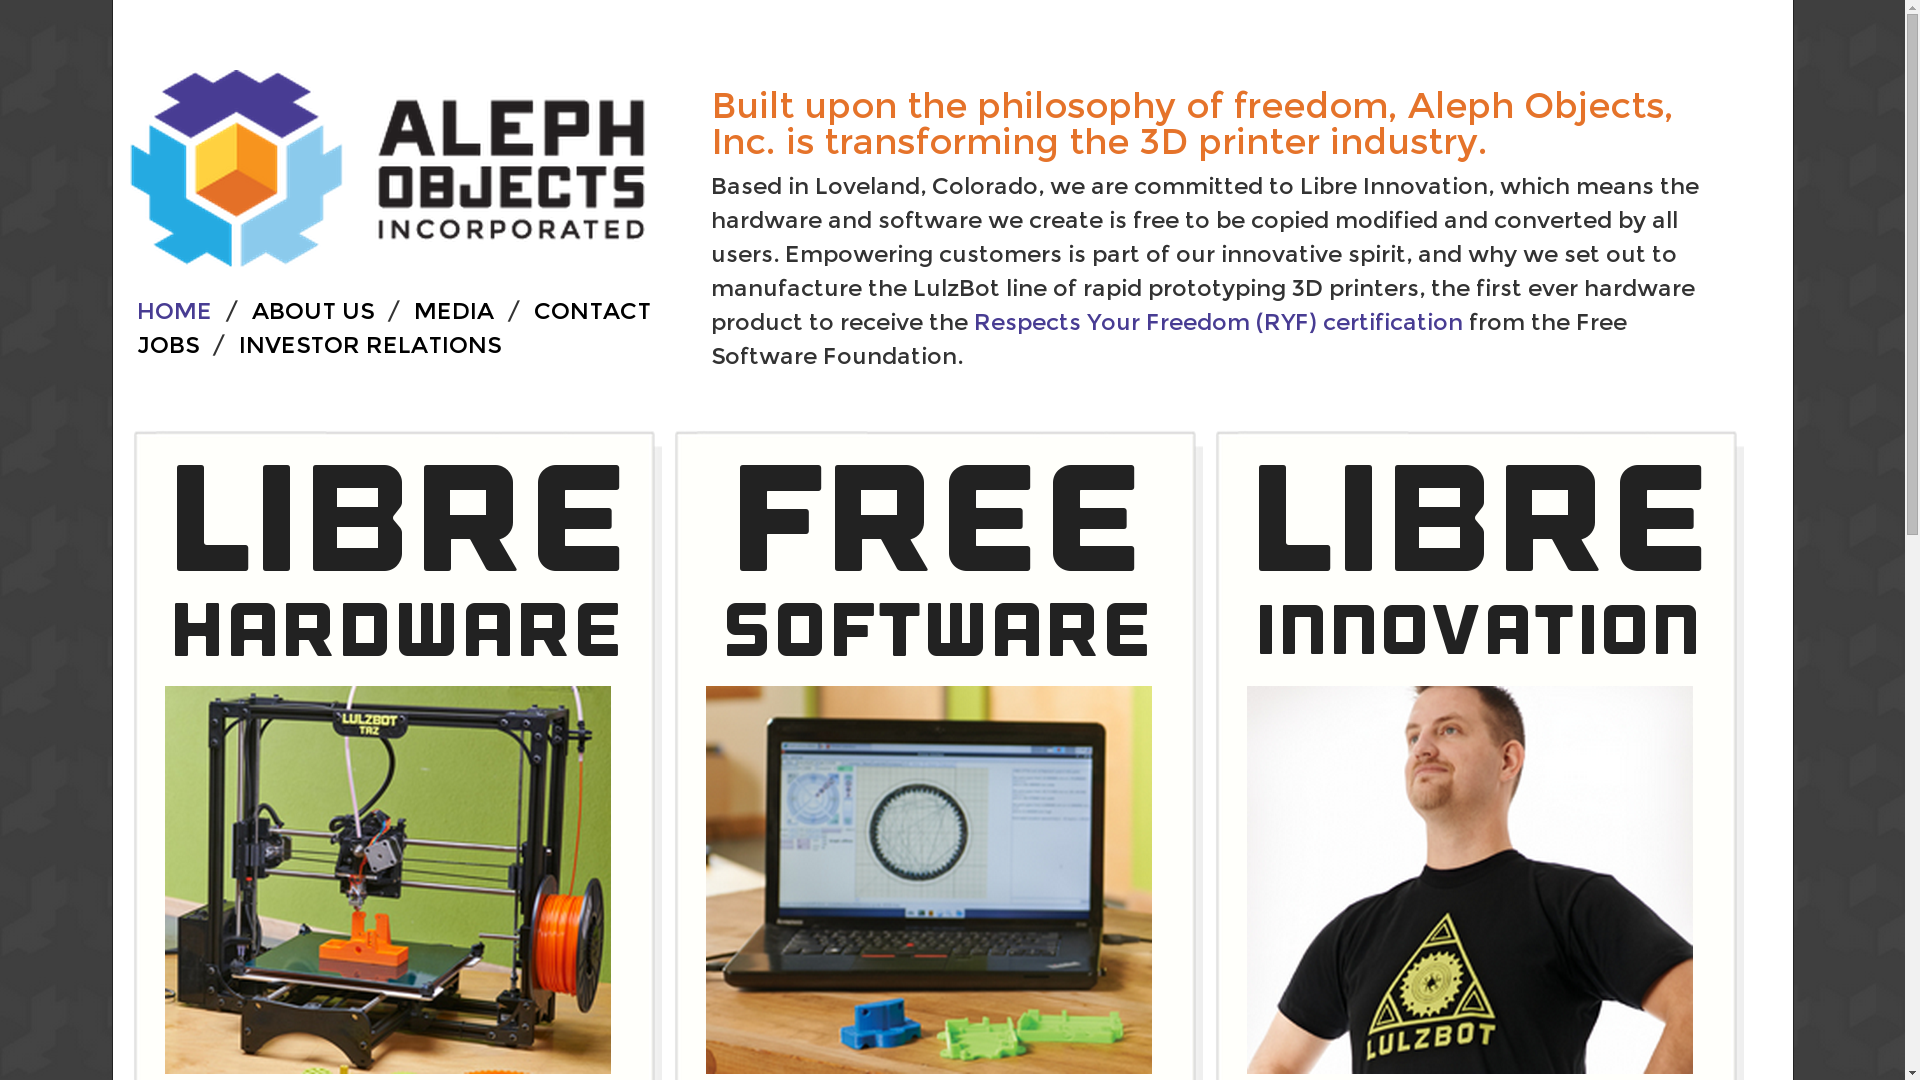
\includegraphics[keepaspectratio=true,height=1.10\textheight,width=1.00\textwidth,angle=0]{www.alephobjects.com.png}
 \caption{Aleph Objects website, \href{www.alephobjects.com}{www.alephobjects.com}}
 \label{fig:wwwalephobjectscom}
\end{figure}

\subsection{LulzBot}
\url{https://www.lulzbot.com} --- Main LulzBot website.
\begin{figure}[h!]
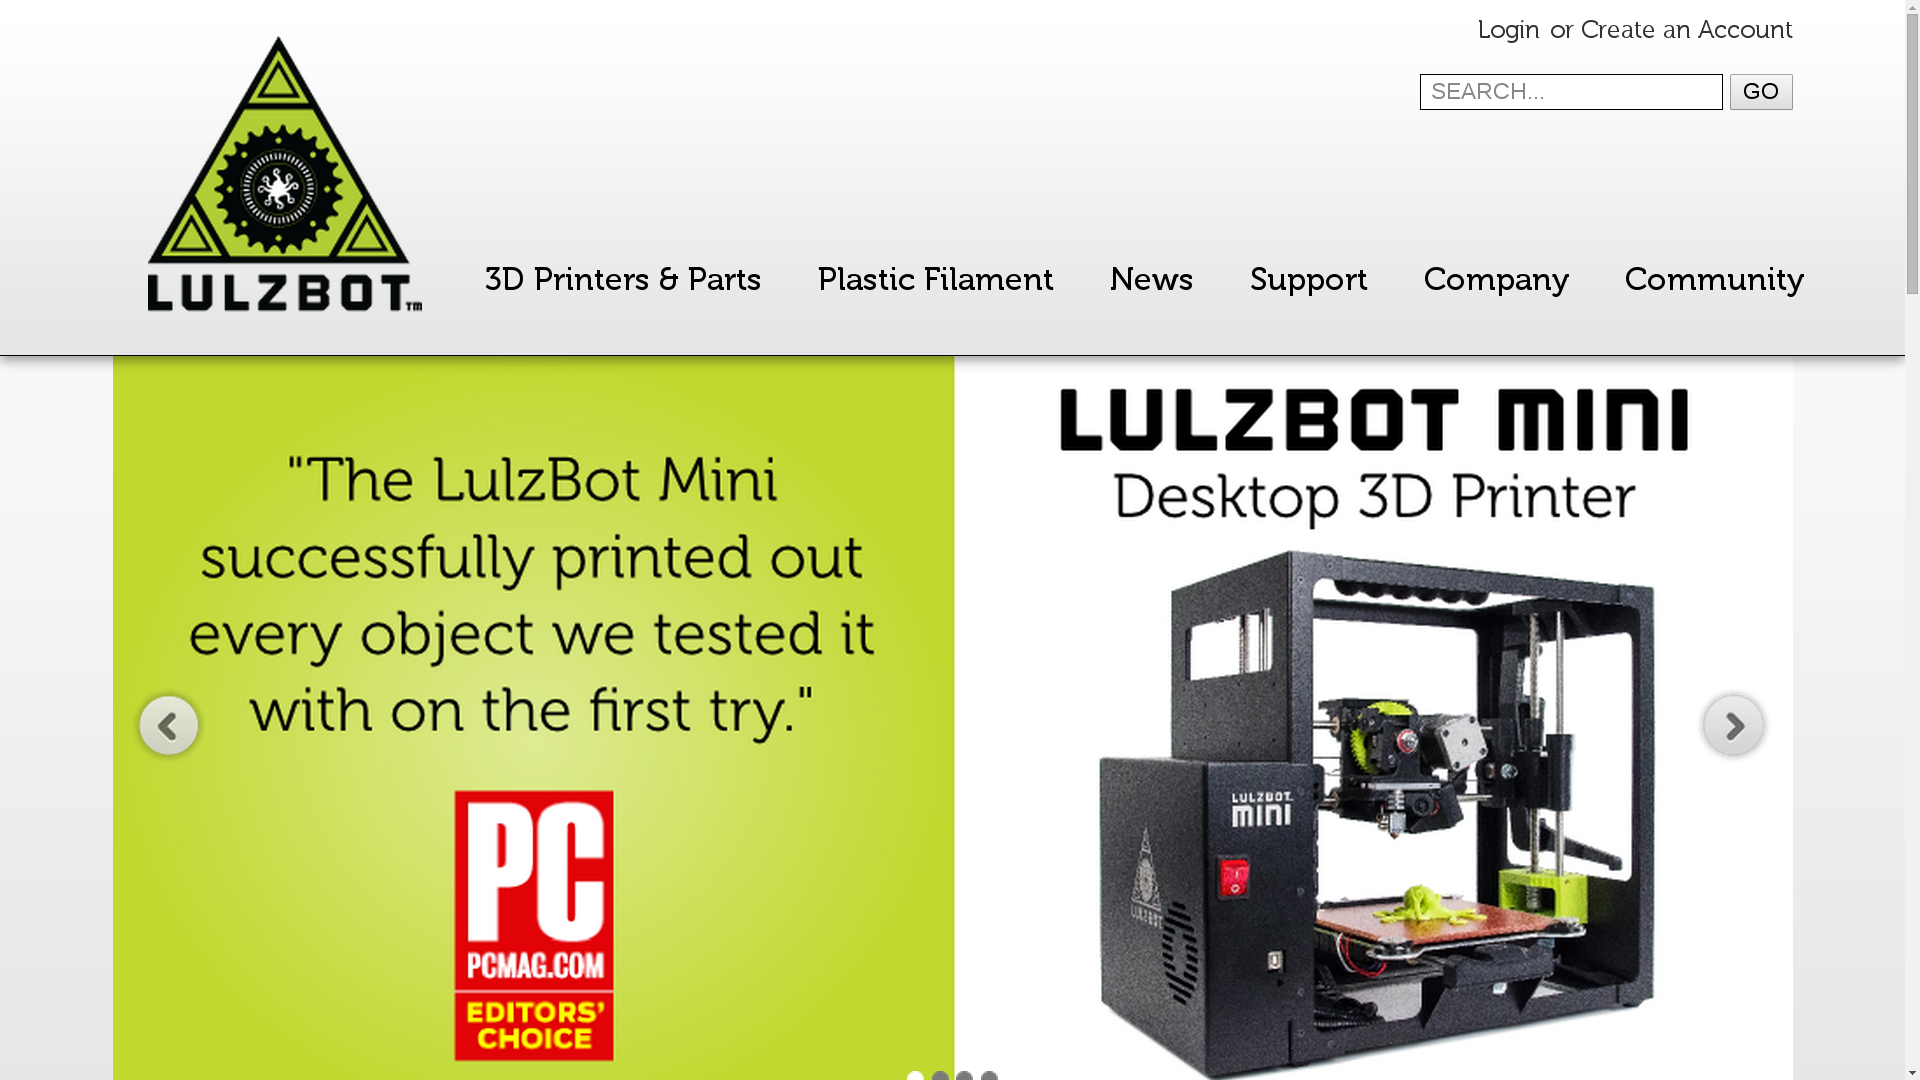
\includegraphics[keepaspectratio=true,height=1.10\textheight,width=1.00\textwidth,angle=0]{www.lulzbot.com.png}
 \caption{LulzBot website, \href{www.lulzbot.com}{www.lulzbot.com}}
 \label{fig:wwwlulzbotcom}
\end{figure}

\subsection{Aleph Objects Development Archive}
\url{https://devel.alephobjects.com} --- Public development files for
Aleph Objects.

\subsection{LulzBot Development Archive}
\url{https://devel.lulzbot.com} --- Public development files for LulzBot.

\subsection{Aleph Objects Software Downloads}
\url{https://download.alephobjects.com} --- Aleph Objects downloads.

\subsection{LulzBot Products Final Release Files}
\url{https://download.lulzbot.com} --- Final release source code for
LulzBot products.

\subsection{LulzBot User Discussion Forum}
\url{https://forum.lulzbot.com} --- User discussion forum for LulzBot.
\begin{figure}[h!]
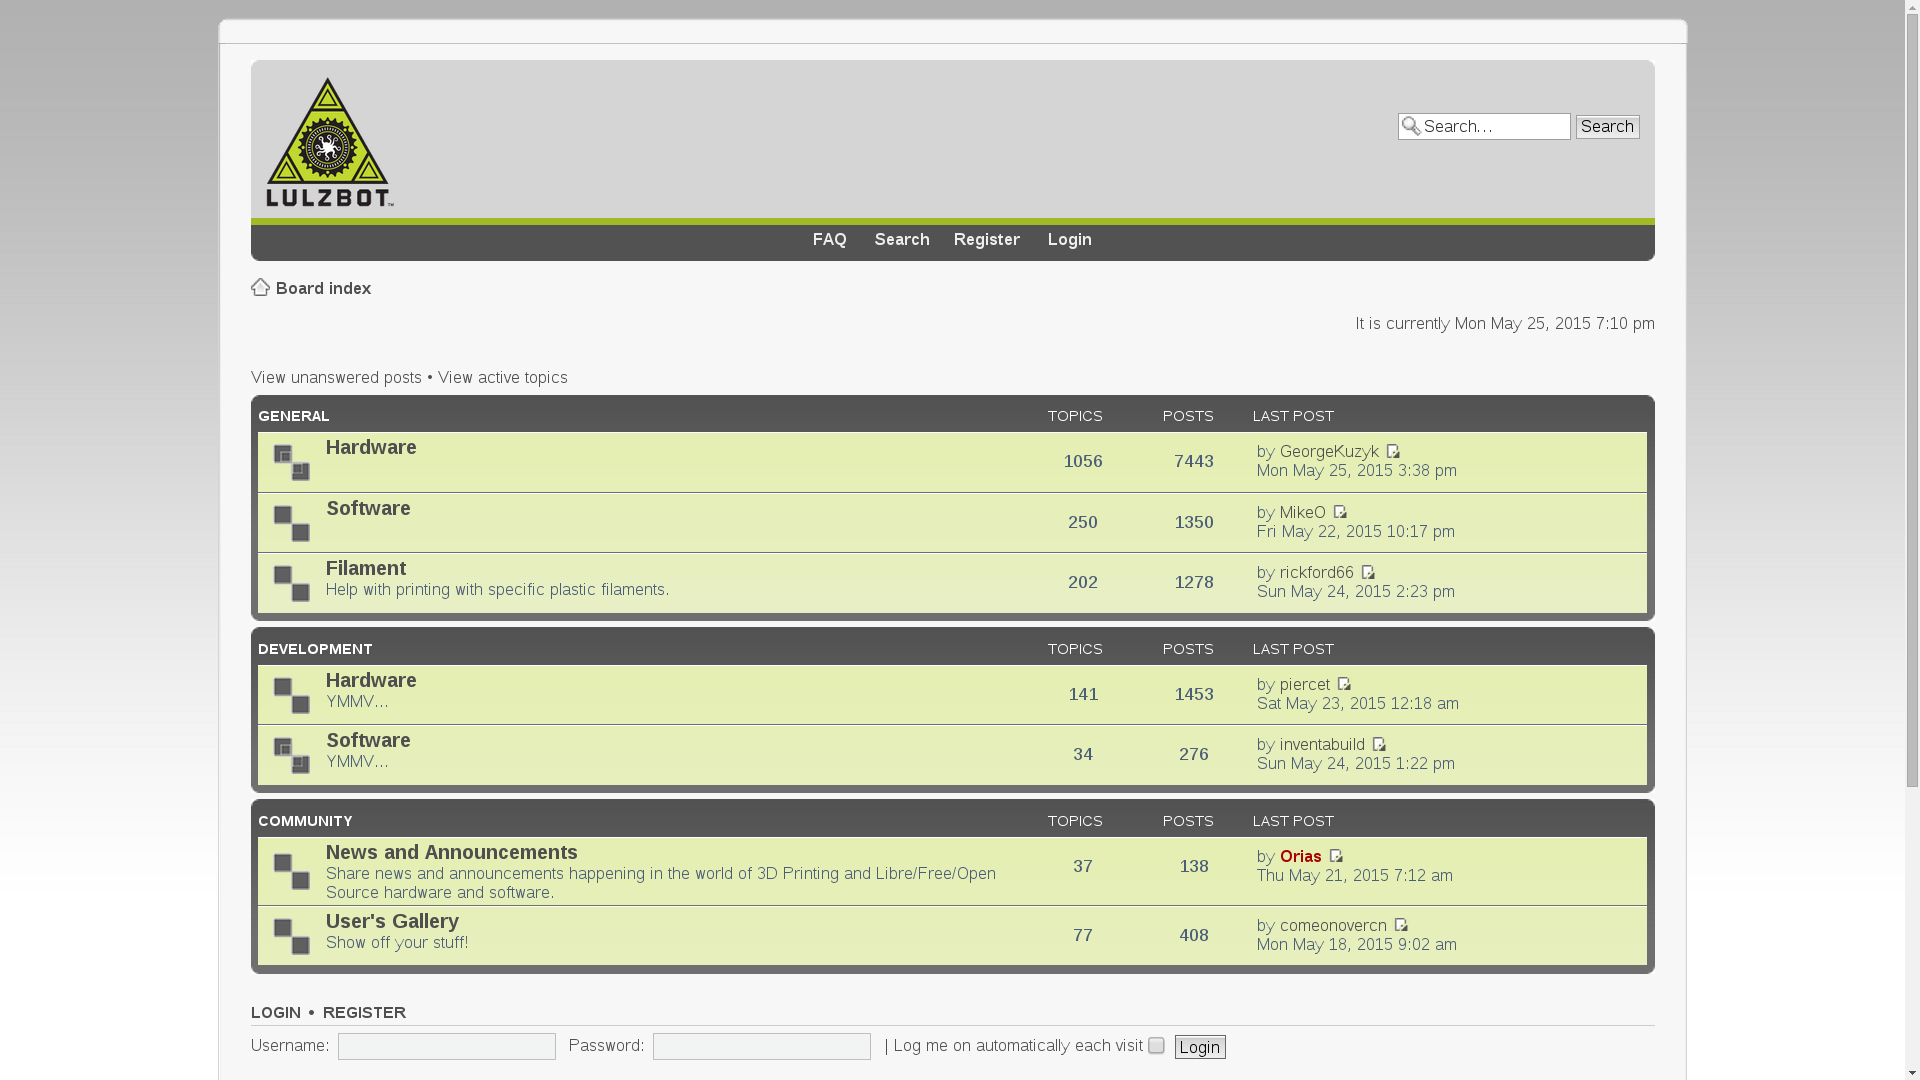
\includegraphics[keepaspectratio=true,height=1.10\textheight,width=1.00\textwidth,angle=0]{forum.lulzbot.com.png}
 \caption{LulzBot user discussion forum, \href{forum.lulzbot.com}{forum.lulzbot.com}}
 \label{fig:forumlulzbotcom}
\end{figure}

\subsection{Open Hardware Assembly Instructions Kit}
\url{https://ohai-kit.alephobjects.com} --- Visual work instructions for
assembling products and user support.
\begin{figure}[h!]
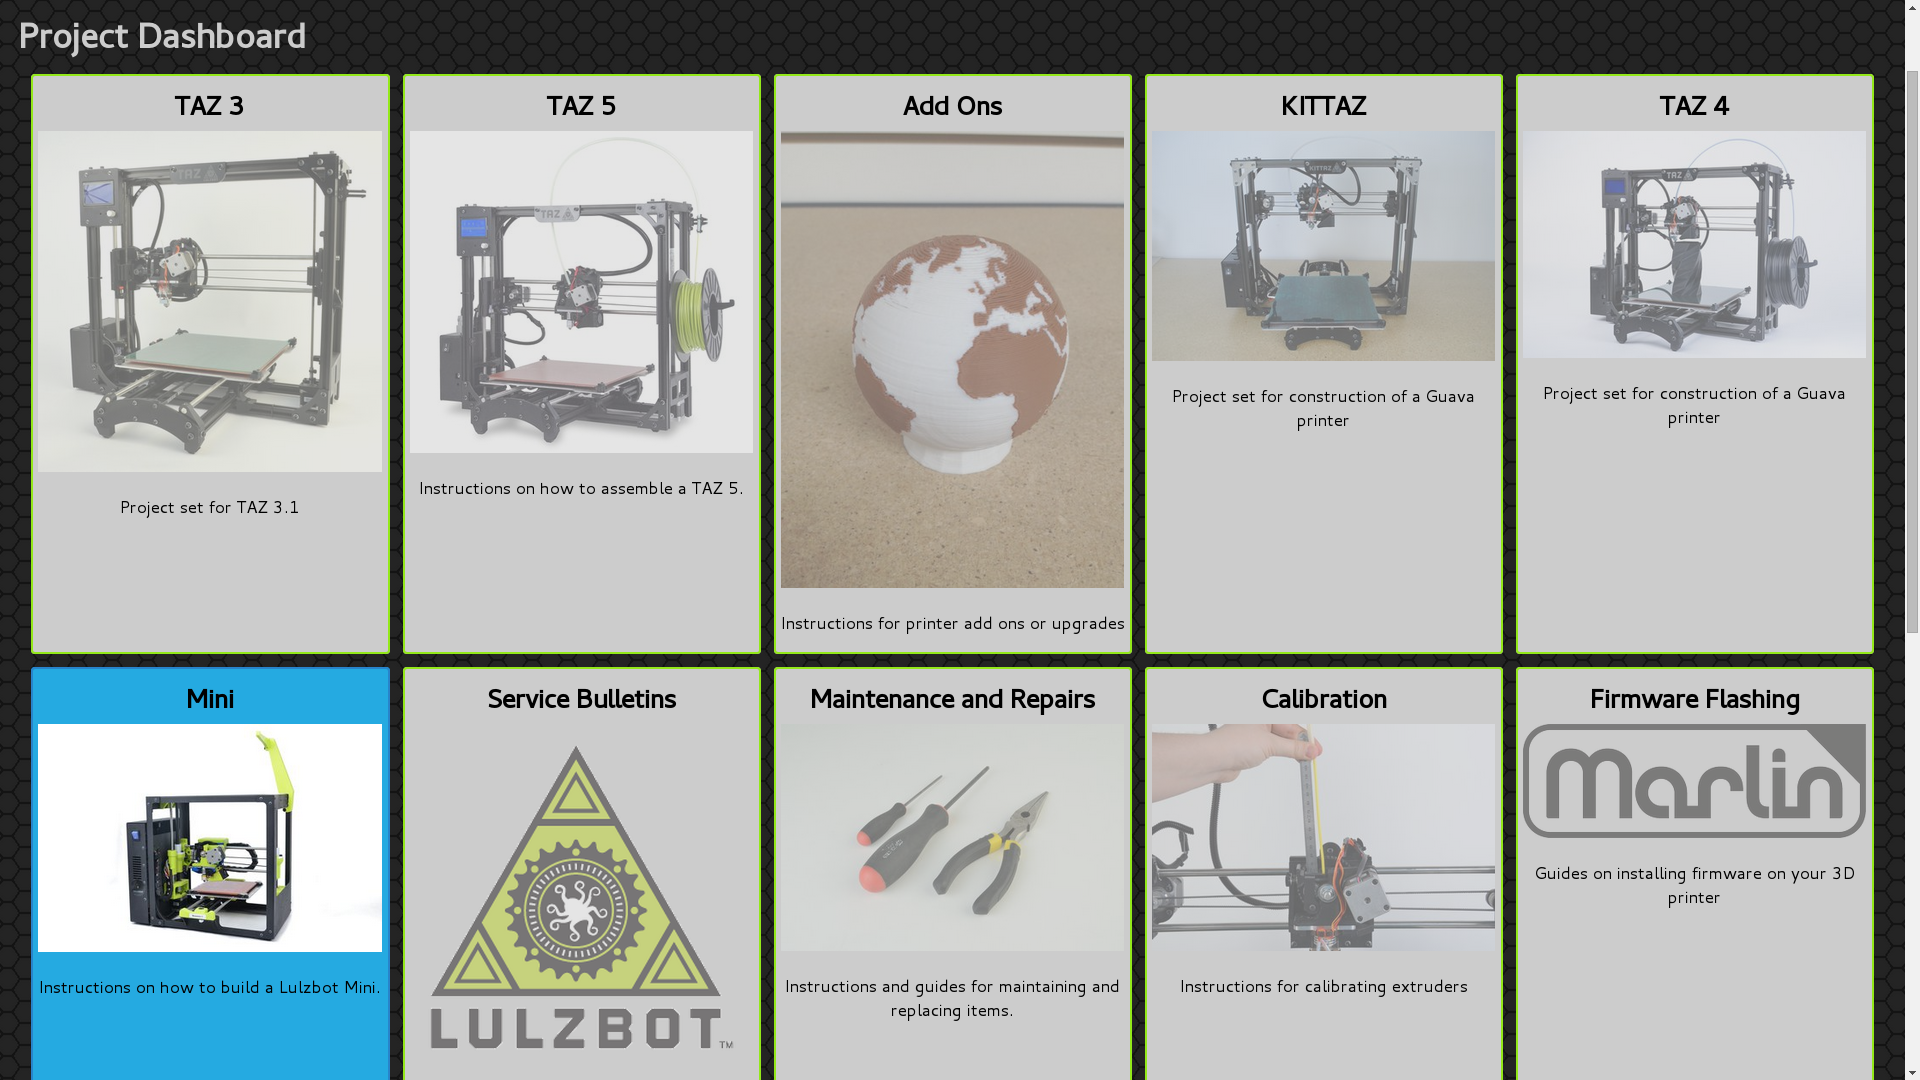
\includegraphics[keepaspectratio=true,height=1.10\textheight,width=1.00\textwidth,angle=0]{ohai-kit.alephobjects.com.png}
 \caption{Open Hardware Assembly Instructions Kit, \href{ohai-kit.alephobjects.com}{ohai-kit.alephobjects.com}}
 \label{fig:ohaikitalephobjectscom}
\end{figure}

\subsection{Newsletter}
\url{https://phplist.alephobjects.com} --- Newletter mailing list.

\subsection{Surveys}
\url{https://survey.alephobjects.com} --- Surveys.

\subsection{Rsync}
\url{rsync://rsync.alephobjects.com} --- Rsync file server of download
and development archives.

